\documentclass[10pt, headsepline, captions=tableabove,xcolor=table]{beamer}
% ==> \documentclass[10pt, handout]{beamer}    to print 4 in one page
\usepackage[utf8]{inputenc}
% \usepackage{multicol}
\usepackage{amsmath}
\usepackage[brazilian]{babel}
\usepackage{xcolor}
\usepackage{fancybox}
\usepackage{pgfpages}
%\usepackage{enumitem}
% ==> \pgfpagesuselayout{4 on 1}[]      to print 4 in one page

\usetheme{Warsaw}
\usecolortheme{default}
\usefonttheme{professionalfonts}
\graphicspath{{./imgs/}}
\setbeamertemplate{caption}[numbered]
\setbeamertemplate{footline}[frame number]
\setbeamercovered{transparent}
\setbeamertemplate{section in toc}{\inserttocsectionnumber.~\inserttocsection} % TOC style
%\setbeamercovered{invisible}
%\geometry{left=1cm, right=1cm, top=0.5cm, bottom=0.5cm}

\title{Lógica Matemática}
\subtitle{Parte 1}
\author[Paulo Pinheiro]
{Dr. Paulo Vinicius Pereira Pinheiro\inst{1}}
\institute[UNIFAP]
{
    \inst{1}
    Centro Universitário Paraíso do Ceará\\
    UNIFAP
}
%
\date{\small{Acesse estes slides em:\\ \url{https://github.com/paulovpp/slides}}\newline \\Última atualização:\\ \today}
\logo{
\includegraphics[height=0.7cm]{imgs/UNIFAP.png}}
%
%%%%%%%%%%%%%%%%%%%%%%%%%%%%%%%%%%%%%%%%%%%%%%%%%%%%%%%%%%%%%%%%%%%%%%%%%%%%%
%
\begin{document}
% \setcounter{tocdepth}{1} % Show sections
% \setcounter{tocdepth}{2} % + subsections
% Title page frame
\begin{frame}
    \titlepage
\end{frame}

% Remove logo from the next slides
\logo{}

% Outline frame
\begin{frame}[t]{Sumário}
    \tableofcontents[sections={1-3}]
\end{frame}
%
\begin{frame}[t]{Sumário}
    \tableofcontents[sections={4-}]
\end{frame}

%% -------------------------------- %% -----------------------------------%%
%% Section 1 - Introductory concepts
\section{Introdução}
%
% \begin{frame}[c]
%     \begin{block}{\LARGE{Definições iniciais}}
%     \end{block}
% \end{frame}
\subsection{Objetivos}
%
\begin{frame}[c]
    \frametitle{Objetivos do curso}
    \framesubtitle{List all course objectives}
    \begin{alertblock}{Estudo da lógica proposicional}
        \begin{itemize}
            \item Representar e especificar os conceitos de sintaxe e semântica associados a qualquer lógica utilizada ou linguagem.
            \item Estudar os métodos que produzem ou verifiquem as fórmulas ou argumentos utilizados.
            \item Definir sistemas de dedução formal onde são consideradas as noções de prova e consequência lógica.
            \item Correlacionar diagramas de Venn com a prática.
            \item Conhecer a álgebra de Boole.
        \end{itemize}
    \end{alertblock}
\end{frame}
%
\subsection{Definições iniciais}
%
\begin{frame}[t]
    \frametitle{Definições iniciais}
    \framesubtitle{Introductory definitions to the course}
    \textbf{Proposição}\\
    \quad $\star$ \textcolor{blue}{É qualquer conjunto de palavras ou símbolos que expressam um pensamento completo.}\\
    \quad $\star$ As proposições transmitem fatos ou exprimem juízos que formamos a respeito de determinado acontecimento.\\ \pause
    \textbf{Exemplos}
    \begin{itemize}
        \item A lua é um satélite da Terra.\pause
        \item O valor arredondado de $\pi$ vale $3,14$.\pause
        \item Recife é a capital da Paraíba\pause
        \item $\cos(90^o)~=~0$.\pause
    \end{itemize}
    \textbf{Alfabeto}\\
    \quad $\star$ É o conjunto de símbolos usado em qualquer linguagem. A seguir a tabela de símbolos usados na disciplina é apresentado:
\end{frame}
%
%% -------------------------------- %% -----------------------------------%%
%% Section 2 - Lógica proposicional - Início 
\section{Lógica proposicional - Início}
%
\subsection{Conceitos iniciais}
%
\begin{frame}[t]
    \frametitle{Conceitos iniciais}
    \framesubtitle{Introductory definitions to start the course}
    \begin{block}<1->{Alfabeto da lógica proposicional}
        \begin{itemize}
            \item Símbolo de pontuação: (,)
            \item Símbolos booleanos: \textit{true, false}
            \item Símbolos proposicionais simples: $p,~q,~r,~s,~p_1,~q_2$
            \item Símbolos proposicionais compostos: $P,~Q,~R,~S,~P_1,~Q_1,~S_2$
            \item Conectivos proposicionais: $\land,~\lor,~\lnot,~\rightarrow, ~\leftrightarrow$
        \end{itemize}
    \end{block}
    %
    \begin{block}<2->{Fórmulas}
        \quad São conjuntos de proposições unidos por um conectivo obtendo um valor booleano como resultante. São construídas a partir dos símbolos do alfabeto proposicional.\\
        \quad \textcolor{red}{Tal como ocorre nas linguagens faladas ou escritas, não é qualquer concatenação de símbolos que é uma fórmula.}
    \end{block}
\end{frame}
%
\begin{frame}[t]
    \pagecolor{black}
    %\color{white}% set the default colour to white
    \frametitle{Algumas definições}
    \framesubtitle{Examples of logic formulas}
        \begin{itemize}
            \item Todo símbolo de verdade $(V)$ é uma fórmula.
            \item Todo símbolo proposicional é uma fórmula.
            \item Se $H$ é uma fórmula então $(\lnot H)$, a negação de $H$, é uma fórmula.
            \item Se $H$ e $G$ são fórmulas então $(H \land G)$, $(H \lor G)$, $(H \rightarrow G)$ e $(H \leftrightarrow G)$ são fórmulas. 
        \end{itemize}
        %
        {\color{blue} \rule{\linewidth}{1mm}}
        \pause
        \textbf{Não são fórmulas:}\\
        \begin{itemize}
            \item $PR$
            \item $(H~true~\leftrightarrow)$
            \item $(true~\rightarrow \leftrightarrow (H~true \rightarrow))$
            \item $PH \rightarrow \land$
            \item $true \rightarrow \lor$
        \end{itemize}
\end{frame}
%
\subsection{Princípios fundamentais da lógica matemática}
%
\begin{frame}
    \frametitle{Princípios da lógica clássica}
    %\framesubtitle{Basic principles compared to fundamental rules to mathematical logic}
    %
    \begin{block}{Princípio da identidade}
        Uma proposição não pode ser verdadeira e falsa ao mesmo tempo. \\
        \center{$P~\text{é igual a}~P$}
    \end{block}
    \pause
    %
    \begin{block}{Princípio da não contradição}
        Uma proposição não pode ser \textit{verdadeira} e \textit{falsa} ao mesmo tempo.
        $$ \text{não}~\left(P~\text{e não}~P\right) $$
    \end{block}
    \pause
    %
    \begin{block}{Princípio do terceiro excluído}
        Toda proposição ou é verdadeira ou é falsa, não existindo um terceiro valor que ela possa assumir.
        $$ P~\text{ou não}~P~(\otimes - \text{ou exclusivo})$$
    \end{block}
\end{frame}
%
\subsection{Tipos de proposições}
%
\begin{frame}
    \frametitle{Proposição simples e compostas}
    \framesubtitle{Simple or compound preposition}
    $\star$ \textbf{Proposições simples}\\
    É aquela que contêm somente uma afirmação.\\
    \textbf{Exemplo:}\\
    \textcolor{teal}{Nós somos ricos.}\\
    \textcolor{teal}{Não como todo dia.}\\
    %
    \hfill \break
    $\star$ \textbf{Proposições compostas}\\
    Uma proposição é dita composta quando for constituída por uma sequência finita de pelo menos duas proposições.\\
    \textbf{Exemplo:}\\
    \textcolor{teal}{Vamos ao cinema ou ao teatro.}\\
    \textcolor{teal}{O céu é azul e cheio de nuvens.}
\end{frame}
%
\subsection{Conectivos proposicionais}
%
\begin{frame}[t]
    \frametitle{Conectivos do cálculo proposicional}
    \framesubtitle{Conectors for all arithmetic with propositions.}
    Na linguagem comum, palavras explícitas são utilizadas ou não para interligar frases dotadas de algum sentido. Tais palavras são substituídas, na \textbf{Lógica Matemática}, por símbolos denominados \textit{conectivos lógicos}.\\
    \hfill \break
    Em nosso estudo, nos restringiremos inicialmente ao chamado \textbf{cálculo proposicional}. Por essa razão, os conectivos utilizados são conhecidos por \textit{sentenciais} ou \textit{proposicionais.}\\
    \hfill \break
    Existem cinco conectivos que substituirão simbolicamente as expressões:
    \begin{itemize}
        \item \textit{e}$~(\land)$ - do inglês \textit{AND}
        \item \textit{ou}$~(\lor)$ - do inglês \textit{OR}
        \item \textit{se ..., então ...}$(\rightarrow)$ - do inglês \textit{IF ... then ...}
        \item \textit{se, e somente se ...}$(\leftrightarrow)$ - do inglês \textit{IF  and ONLY IF ...}
        \item \textit{não}$~(\lnot)$ - do inglês \textit{NOT}
    \end{itemize}
\end{frame}
%
\begin{frame}[t]
    \small
    \frametitle{Conectivos do cálculo proposicional}
    \framesubtitle{Examples}
    %
    \begin{exampleblock}{Exemplo 1}
        \textbf{Somos pobres mortais e fanáticos torcedores da vida.}\\[2pt]
        É uma proposição composta:\\[2pt]
        \textbf{1a proposição:} somos pobres mortais, \\[2pt]
        \textbf{2a proposição:} somos fanáticos torcedores da vida, \\[2pt]
        \textbf{Conectivo:} e (\textit{AND})
    \end{exampleblock}
    %
    \begin{exampleblock}{Exemplo 2}
        \textbf{Se não nos alimentarmos, morremos.}\\[2pt]
        É uma proposição composta:\\[2pt]
        \textbf{1a proposição:} nos alimentarmos, \\[2pt]
        \textbf{2a proposição:} (nós) morreremos, \\[2pt]
        \textbf{Conectivo:} Se ..., então ...
    \end{exampleblock}
\end{frame}
%
%% -------------------------------- %% -----------------------------------%%
%% Section 3 - Lógica proposicional - cálculo proposicional
\section{Lógica proposicional - cálculo proposicional}
%
\subsection{Tabela verdade}
%
\begin{frame}[t]
    \frametitle{Tabela verdade}
    \framesubtitle{True table of operators}
    %
    \begin{alertblock}{Definição}
        \small
        Segundo o princípio do \textbf{terceiro excluído}, toda proposição simples $p$ ou composta $H(p,q,...)$ só pode assumir \textbf{valor lógico} igual a \\ [1pt]
        \center{$V$ (verdade - \textit{TRUE}) \qquad ou \qquad  $F$ (falsidade - \textit{FALSE})} \\ [4pt]
        A \textbf{tabela-verdade} sintetiza o resultado de funções lógicas para $n$ proposições.
    \end{alertblock}
    %
    \vspace{-4mm}
    %
    \begin{figure}[c]
        \centering
        \caption{Tabela verdade para um estado(proposição) único.}
        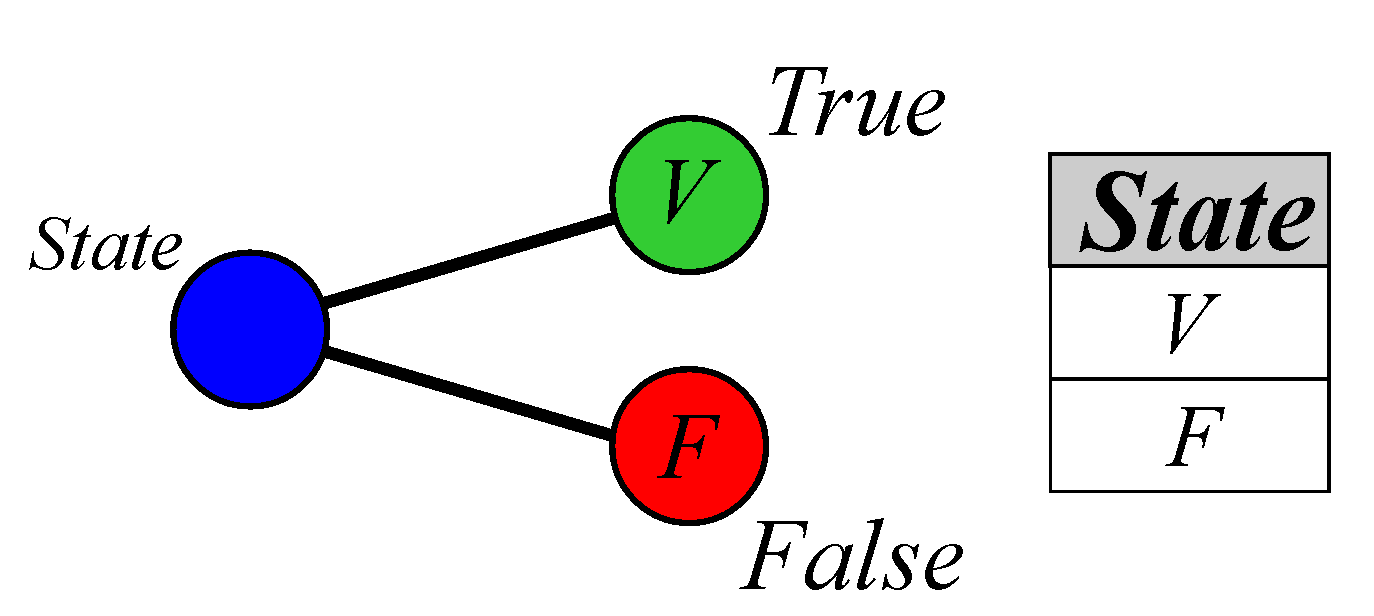
\includegraphics[scale=0.25]{TT2.png}
        \label{fig:tabela-verdade1}         
    \end{figure}
\end{frame}
%
\begin{frame}[c]
    \frametitle{Tabela verdade}
    \framesubtitle{Examples}
    %
    \begin{figure}[c]
        \centering
        \caption{Tabela verdade para uma proposição composta $H(p,q)$.}
        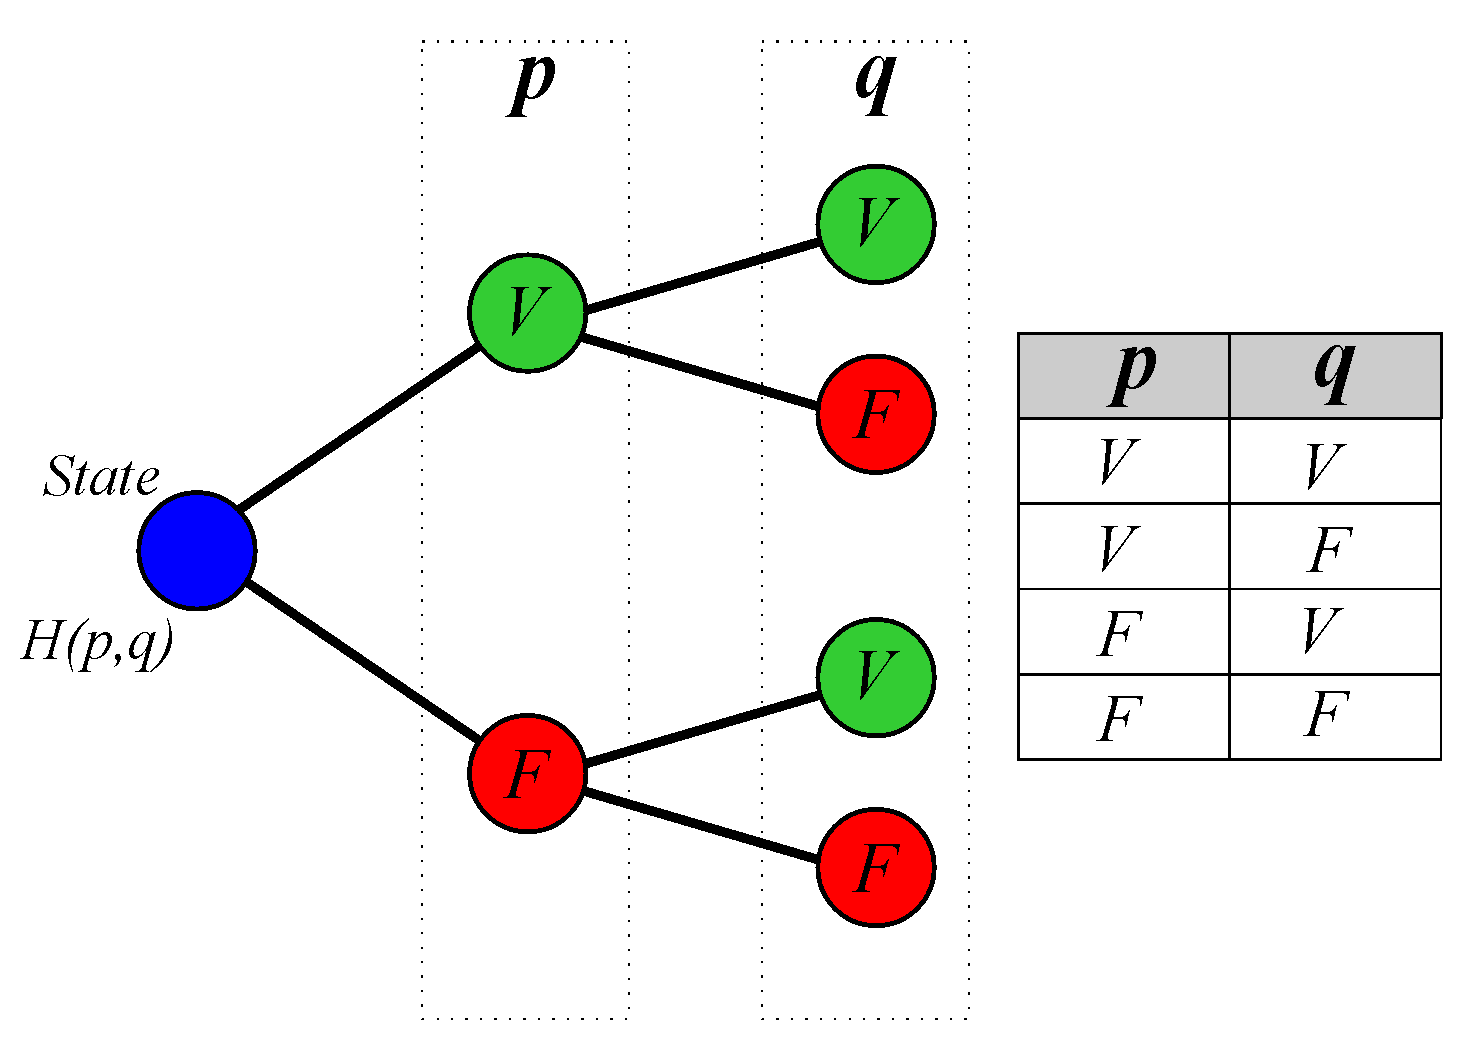
\includegraphics[scale=0.30]{TT3.png}
        \label{fig:tabela-verdade2}
    \end{figure}
\end{frame}
%
\begin{frame}[c]
    \frametitle{Tabela verdade}
    \framesubtitle{Examples}
    %
    \begin{figure}[c]
        \centering
        \caption{Tabela verdade para uma proposição composta $H(p,q,r)$.}
        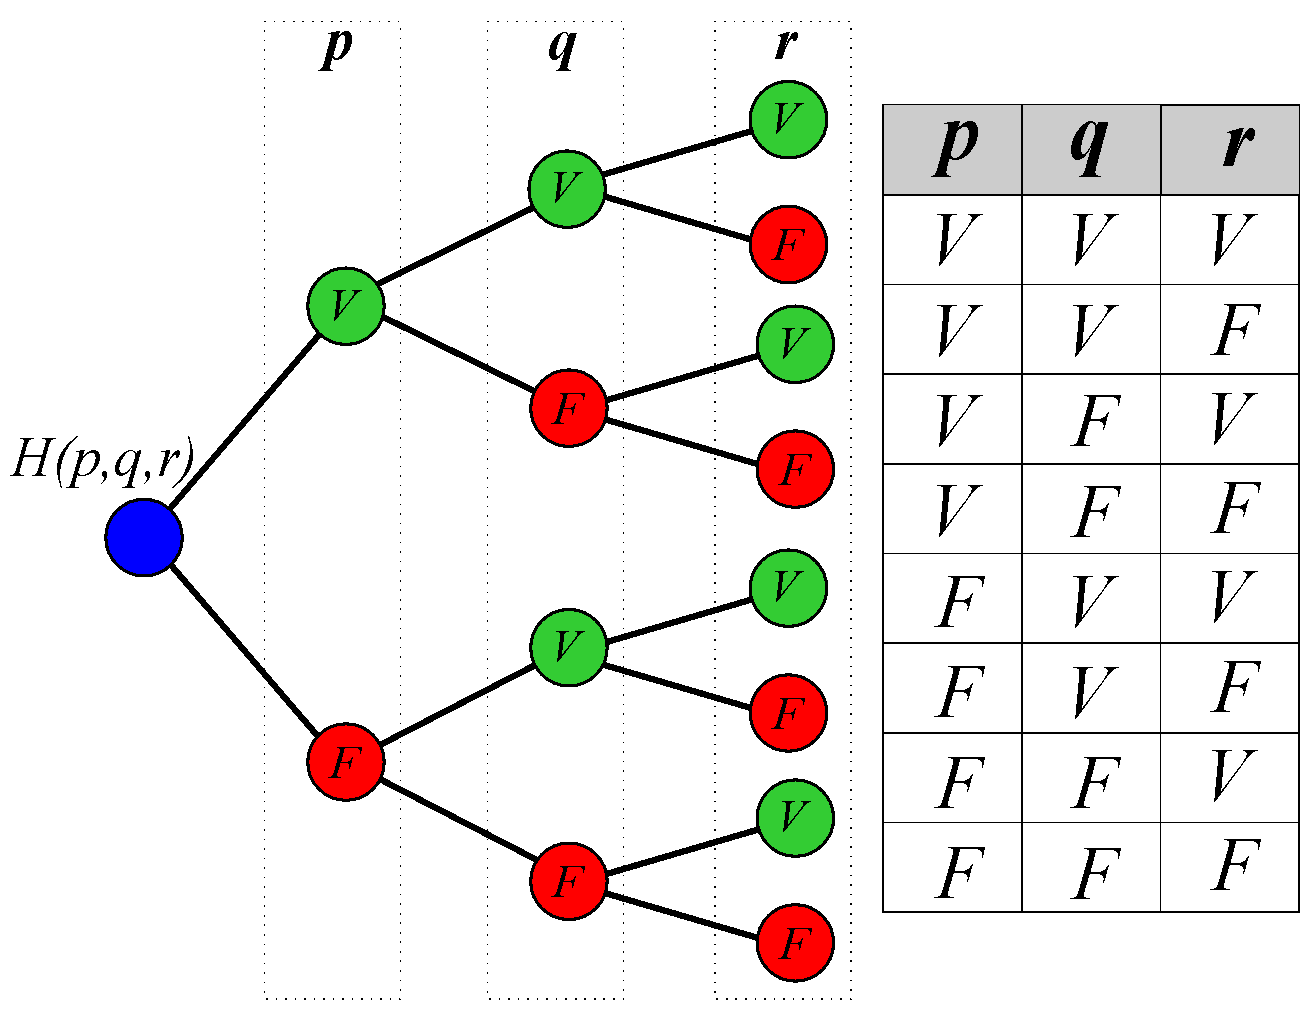
\includegraphics[scale=0.30]{TT4.png}
        \label{fig:tabela-verdade3}
    \end{figure}
\end{frame}
%
\subsection{Ordem de precedência e comprimento de fórmulas}
%
\begin{frame}[t]
    \frametitle{Definições complementares}
    \framesubtitle{Final considerations of the section - Procedence order}
    %
    \small
    \begin{block}{Ordem de precedência}
        \begin{itemize}
            \item Maior precedência: $\lnot$ ou $\sim$ 
            \item Precedência intermediária: $\rightarrow$ e $\leftrightarrow$
            \item Menor precedência: $\land$ e $\lor$
        \end{itemize}        
    \end{block}
    \pause
    \begin{block}{Comprimento de uma fórmula}
        \begin{itemize}
            \item Se $H$ é um símbolo proposicional ou de verdade então $comp[H]=1$
            \item Se $H$ e $G$ são fórmulas da \textbf{lógica proposicional}, então
        \end{itemize}
        %\vspace{-3mm} % if negative it removes vertical space
        \begin{gather*}
            comp[\lnot H] = comp[H] + 1 \\
            comp[H \land G]~\text{ ou }~comp[H \lor G] = comp[H] + comp[G] + 1 \\
            comp[H \rightarrow G]~\text{ ou }~comp[H \leftrightarrow G] = comp[H] + comp[G] + 1
        \end{gather*}
        % gather environment: align equations on center
    \end{block}
\end{frame}
%
\subsection{Valor lógico}
%
\begin{frame}[t]
    \frametitle{Definições finais}
    \framesubtitle{Final considerations of the section 2/2}
    \small
    \begin{block}{Valor lógico}
        O \textbf{valor lógico} de uma proposição simples ou composta expressa seu valor resultante se \textit{verdadeiro} ou \textit{falso}.
        \begin{itemize}
            \item Para uma proposição simples $p$, $V(p)$ expressa seu valor lógico.
            \item Para uma proposição composta $H$, $V(H)$ expressa seu valor lógico.
        \end{itemize}
    \end{block}
        %
    \begin{columns}[T]
        \begin{column}{.5\textwidth}
            \begin{exampleblock}{Exemplo 1}
                \quad $p$ : O sol é verde. \\
                \quad $q$ : O sol é quente. \\
                \quad $r$ : O mar não é vermelho.\\[4pt]
                \quad $V(p) = V$, $V(q) = F$, $V(\lnot r)=F$ \\
                \quad $V(p \land q) = F$, \quad $V(q \lor r) = V$
            \end{exampleblock}
        \end{column}
        %
        %\hspace{5mm}
        \begin{column}{.5\textwidth}
            \begin{exampleblock}{Exemplo 2}
                \quad $p_1$ : $x \geq 10$   \\
                \quad $p_2$ : $x < 50$\\
                \quad $p_3$ : $x > 25$ \\[4pt]
                $V(p_1) = V$, $V(p_2) = F$, $V(\lnot p_3)=F$ \\
                \quad $V(p_1 \land p_2) = V$, $V(p_3 \land p_2) = F$
            \end{exampleblock}
        \end{column}
    \end{columns}
\end{frame}
%
\subsection{Exercícios}
%
\begin{frame}[t] % \renewcommand{\theenumi}{\alph{enumii}}
    \frametitle{Exercícios - 1/2}
    \framesubtitle{Practice the chapters concepts}
    %
    \small
    \setbeamercovered{invisible}
    \setbeamercolor{enumerate item}{fg=red!80!black}
    \setbeamertemplate{enumerate items}[default]
    \begin{exampleblock}{1. Identifique os itens abaixo que não são fórmulas da lógica proposicional.}
        \begin{columns}[T]
            \begin{column}{0.15\textwidth}
                \begin{enumerate}[\bf a.]
                    \item $pq$
                    \item $PQ$
                    \item $PQ \lnot$
                    \item $\lnot PQ$
                \end{enumerate}
            \end{column}
            %
            \hspace*{-5mm}
            %
            \begin{column}{0.15\textwidth}
                \begin{enumerate}[\bf a.]
                    \addtocounter{enumi}{4}
                    \item $p \land q$
                    \item $P \lor Q$
                    \item $PQ \land$
                    \item $\lor PQ$
                \end{enumerate}
            \end{column}
            %
            \hspace*{-5mm}
            %
            \begin{column}{0.20\textwidth}
                \begin{enumerate}[\bf a.]
                    \addtocounter{enumi}{8}
                    \item $p \rightarrow q$
                    \item $PQ \rightarrow$
                    \item $\rightarrow PQ \lnot$
                    \item $P \rightarrow Q \rightarrow $
                \end{enumerate}
            \end{column}
            %
            \hspace*{-7mm}
            %
            \begin{column}{0.2\textwidth}
                \begin{enumerate}[\bf a.]
                    \addtocounter{enumi}{12}
                    \item $P \rightarrow Q$
                    \item $P \leftrightarrow Q$
                    \item $P \leftrightarrow q$
                    \item $\leftrightarrow P \leftrightarrow Q$
                \end{enumerate}
            \end{column}
            %
            \hspace*{-8mm}
            %
            \begin{column}{0.25\textwidth}
                \begin{enumerate}[a.]
                    \addtocounter{enumi}{16}
                    \item $P \rightarrow true$
                    \item $P \land true$
                    \item $true~P \leftrightarrow q$
                    \item $false~PQ \land$
                \end{enumerate}
            \end{column}
        \end{columns}
    \end{exampleblock}
    %
    \pause
    \vspace{-2mm}
    %
    \begin{alertblock}{Respostas}
        a, b, c, d, g, h, j, k, l, p, q, s, t
    \end{alertblock}
    %
    \pause
    \vspace{-2mm}
    %
    % \setbeamercolor{enumerate item}{fg=red!80!black}
    % \setbeamertemplate{enumerate items}[default]
    \begin{exampleblock}{2. Determine o comprimento das fórmulas a seguir.}
        \begin{columns}[T]
            \begin{column}{0.8\textwidth}
                \begin{enumerate}[\bf a.]
                    \item $((\lnot \lnot~P \land Q) \leftrightarrow (P \rightarrow Q)) \land~true$
                    \item $(\lnot P \rightarrow (Q \lor R)) \leftrightarrow ((P \land Q) \leftrightarrow (\lnot \lnot R \lor \lnot P))$
                    \item $((P \lor Q) \rightarrow (P \rightarrow (\lnot Q)))$
                \end{enumerate}
            \end{column}
            %
            \pause
            %
            \begin{column}{0.2\textwidth}
                \begin{enumerate}[\bf a.]
                    \item 11
                    \item 13
                    \item 8
                \end{enumerate}
            \end{column}
        \end{columns}
    \end{exampleblock}
\end{frame}
%
\begin{frame}[t] % \renewcommand{\theenumi}{\alph{enumii}}
    \frametitle{Exercícios - 2/2}
    \framesubtitle{Practice the chapters concepts}
    %
    \small
    \setbeamercolor{enumerate item}{fg=red!80!black}
    \setbeamertemplate{enumerate items}[default]
    \begin{exampleblock}{3. Pesquise na internet as proposições para os problemas abaixo.}
        E, se possível, elabore a fórmula para avaliar um valor qualquer.\\
        \begin{enumerate}[\bf P1.]
            \item Verificar se um número $n \in \mathbb{Z} $ está no intervalo $\{n_1, n_2\}$ onde $n_1 > n_2$.
            \item Descobrir o maior entre 2 números.
            \item Descobrir o maior entre 3 números.
            \item Ordenar 2 números.
            \item Ordenar 3 números.
            \item Avaliar se um número é primo.
            \item Buscar letra em palavra (string).
            \item Transformar um tempo dado em \textbf{HH:mm:ss} em apenas \textbf{ss}.
        \end{enumerate}
    \end{exampleblock}
    %
    \normalsize
    \center{\textcolor{red}{\textbf{Trazer na próxima aula para tira-dúvidas.}}}
    \end{frame}
%
%%% -------------------------------- %% -----------------------------------%%
% Section 4 - Fundamental operations under logic propositions
%
\section{Operações lógicas com proposições}
%
\begin{frame}[c]
    \frametitle{Operações lógicas}
    \framesubtitle{Logical operation with propositions}
    %
    \textbf{Operadores da lógica proposicional}\\[2pt]
    \textcolor{green!50!black}{\textbf{Quando pensamos, inerentemente ao processo estamos efetuando inúmeras operações com proposições em nossa mente. Sempre na intenção de formar um raciocínio que nos faça sentido e que possa ser solução para um determinado problema.}}\\[6pt]

    \textcolor{red}{\textbf{As operações lógicas acontecem exatamente com os conectivos proposicionais. Na literatura é comum as duas nomenclaturas se confundirem.}}\\[6pt]
    
    Neste curso, usaremos a notação de \textbf{OPERADORES}. A seguir, as operações lógicas e seus descritivos serão apresentados.

\end{frame}
%
\subsection{Negação}
%
\begin{frame}[t]
    \frametitle{Operação de negação $(\lnot)$ ou $(\sim)$}
    \framesubtitle{Logical NOT operator}
    %
    \begin{block}{Definição}
        Este conectivo não liga duas proposições, mas simplesmente nega a afirmação da proposição que o precede. Em virtude disso, é um conectivo unário, enquanto os anteriores são conectivos binários, pois ligam duas proposições.
    \end{block}
    %
    \vspace{-4mm}
    %
    \begin{columns}[t]
        \begin{column}{0.6\textwidth}
            \begin{exampleblock}{Exemplos}
                Se $V(p) = V$, $\lnot p = F$ \\ [2pt]
                $V(\lnot p) = \lnot V(p)$ \\ [2pt]
                $p:~2+3=5\quad (V)$ e $\lnot p:~2+3 \neq 5\quad (F)$ \\ [2pt]
                $q:~23 < 10 \quad (F)$ e $\lnot q:~23 \nless 10 \quad (V)$ \\[2pt]
                $q:$ Carlos é mecânico. \\[2pt]
                $\lnot q:$ Carlos NÃO é mecânico.
            \end{exampleblock}
        \end{column}
        %
        \hspace{-3mm}
        %
        \begin{column}{0.4\textwidth}
            \begin{table}[t]
                \caption{Tabela verdade $(\lnot)$.}
                \label{tab:tabela-not}
                \begin{tabular}{|c|c|}
                \hline
                \rowcolor[HTML]{EFEFEF} 
                \textbf{$~$p} & \textbf{$\sim$p} \\ \hline
                V          & F                \\ \hline
                F          & V                \\ \hline
                \end{tabular}
            \end{table}
        \end{column}
    \end{columns}
\end{frame}
%
\subsection{Conjunção}
%

\begin{frame}[t]
    \frametitle{Operação de conjunção ($\land$ - 'e' lógico)}
    \framesubtitle{Logical AND operation}
    % 
    \begin{block}{Definição}
        É o resultado da combinação de duas proposições ligadas pela palavra \textbf{e}, que será substituída pelo símbolo $(\land)$. Seu \textbf{valor lógico} somente será VERDADEIRO quando \emph{TODAS} as proposições tiverem seus \textbf{valores lógicos} iguais a VERDADE.
    \end{block}
    \vspace{-4mm}
    %
    \begin{columns}[t]
        \begin{column}{0.6\textwidth}
            \begin{exampleblock}{Exemplos}
                Se $V(p) = V$, $\lnot p = F$ \\ [2pt]
                $V(\lnot p) = \lnot V(p)$ \\ [2pt]
                $p:~2+3=5\quad (V)$ e $\lnot p:~2+3 \neq 5\quad (F)$ \\ [2pt]
                $q:~23 < 10 \quad (F)$ e $\lnot q:~23 \nless 10 \quad (V)$ \\[2pt]
                $q:$ Carlos é mecânico. \\[2pt]
                $\lnot q:$ Carlos NÃO é mecânico.
            \end{exampleblock}
        \end{column}
        %
        \hspace{-3mm}
        %
        \begin{column}{0.4\textwidth}
            \begin{table}[]
                \caption{Tabela verdade $(\land)$.}
                \label{tab:table-and}
                \begin{tabular}{|c|c|c|}
                \hline
                \rowcolor[HTML]{EFEFEF} 
                \textbf{p} & \textbf{q} & \textbf{$p \land q$} \\ \hline
                $V$          & $V$          & $V$                    \\ \hline
                $V$          & $F$          & $F$                    \\ \hline
                $F$          & $V$          & $F$                   \\ \hline
                $F$          & $F$          & $F$                    \\ \hline
                \end{tabular}
            \end{table}
        \end{column}
    \end{columns}
\end{frame}
%
\subsection{Disjunção}
%
\begin{frame}[t]
    \frametitle{Operação de disjunção ($\lor$ - 'ou' lógico)}
    \framesubtitle{Logical OR operator}
    %
    \begin{block}{Definição}
        Este conectivo não liga duas proposições, mas simplesmente nega a afirmação da proposição que o precede. Em virtude disso, é um conectivo unário, enquanto os anteriores são conectivos binários, pois ligam duas proposições.
    \end{block}
    %
    \vspace{-4mm}
    %
    \begin{columns}[t]
        \begin{column}{0.6\textwidth}
            \begin{exampleblock}{Exemplos}
                Se $V(p) = V$, $\lnot p = F$ \\ [2pt]
                $V(\lnot p) = \lnot V(p)$ \\ [2pt]
                $p:~2+3=5\quad (V)$ e $\lnot p:~2+3 \neq 5\quad (F)$ \\ [2pt]
                $q:~23 < 10 \quad (F)$ e $\lnot q:~23 \nless 10 \quad (V)$ \\[2pt]
                $q:$ Carlos é mecânico. \\[2pt]
                $\lnot q:$ Carlos NÃO é mecânico.
            \end{exampleblock}
        \end{column}
        %
        \hspace{-3mm}
        %
        \begin{column}{0.4\textwidth}
            \begin{table}[t]
                \caption{Tabela verdade $(\lnot)$.}
                \label{tab:tabela-ou}
                \begin{tabular}{|c|c|}
                \hline
                \rowcolor[HTML]{EFEFEF} 
                \textbf{$~$p} & \textbf{$\sim$p} \\ \hline
                V          & F                \\ \hline
                F          & V                \\ \hline
                \end{tabular}
            \end{table}
        \end{column}
    \end{columns}
\end{frame}
%
\subsection{Condicional}
%
\subsection{Bicondicional}
%

\begin{frame}{Blocks in Beamer}
    \begin{block}{Standard Block}
        This is a standard block.
    \end{block}
    \begin{alertblock}{Alert Message}
        This block presents alert message.
    \end{alertblock}
    \begin{exampleblock}{An example of typesetting tool}
        Example: MS Word, \LaTeX{}
    \end{exampleblock}
\end{frame}
%
\begin{frame}{Lists in Beamer}

    This is an unordered list:
    \begin{itemize}
        \item Item 1
        \item Item 2
        \item Item 3
    \end{itemize}
    
    and this is an ordered list:
    \begin{enumerate}
        \item Item 1
        \item Item 2
        \item Item 3
    \end{enumerate}
    
    \end{frame}

\end{document}